% Name: Half twist
% Description: The Garside element Δ = σ₁σ₂σ₃σ₁σ₂σ₁ on four strands, which reverses their order, with each strand numbered at both ends.
% Tags: half twist, Garside element, braid group, permutation

\usetikzlibrary{braids}

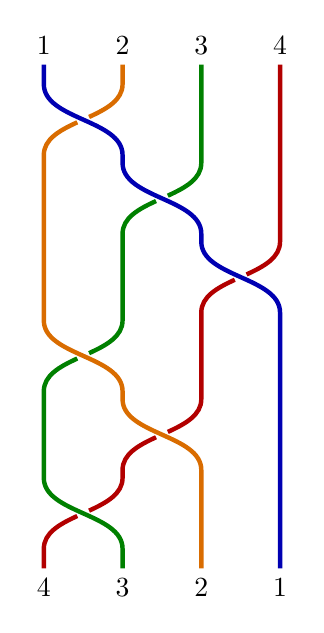
\begin{tikzpicture}
  \pic[
    braid/.cd,
    every strand/.style={ultra thick},
    strand 1/.style={blue!70!black},
    strand 2/.style={orange!85!black},
    strand 3/.style={green!50!black},
    strand 4/.style={red!70!black},
    border height=2mm,
  ] (d) {braid={s_1 s_2 s_3 s_1 s_2 s_1}};
  \foreach \i in {1,...,4} {
    \node[above] at (d-\i-s) {$\i$};
    \node[below] at (d-\i-e) {$\i$};
  }
\end{tikzpicture}
